%-----------------------------------------------------------------------------------------------%
%
% Maret 2019
% Template Latex untuk Tugas Akhir Program Studi Sistem informasi ini
% dikembangkan oleh Inggih Permana (inggihjava@gmail.com)
%
% Template ini dikembangkan dari template yang dibuat oleh Andreas Febrian (Fasilkom UI 2003).
%
% Orang yang cerdas adalah orang yang paling banyak mengingat kematian.
%
%-----------------------------------------------------------------------------------------------%

\chapter*{DAFTAR RIWAYAT HIDUP}
\pagestyle{empty}

\noindent
\begin{wrapfigure}{l}{3cm}\vspace{-15pt}
	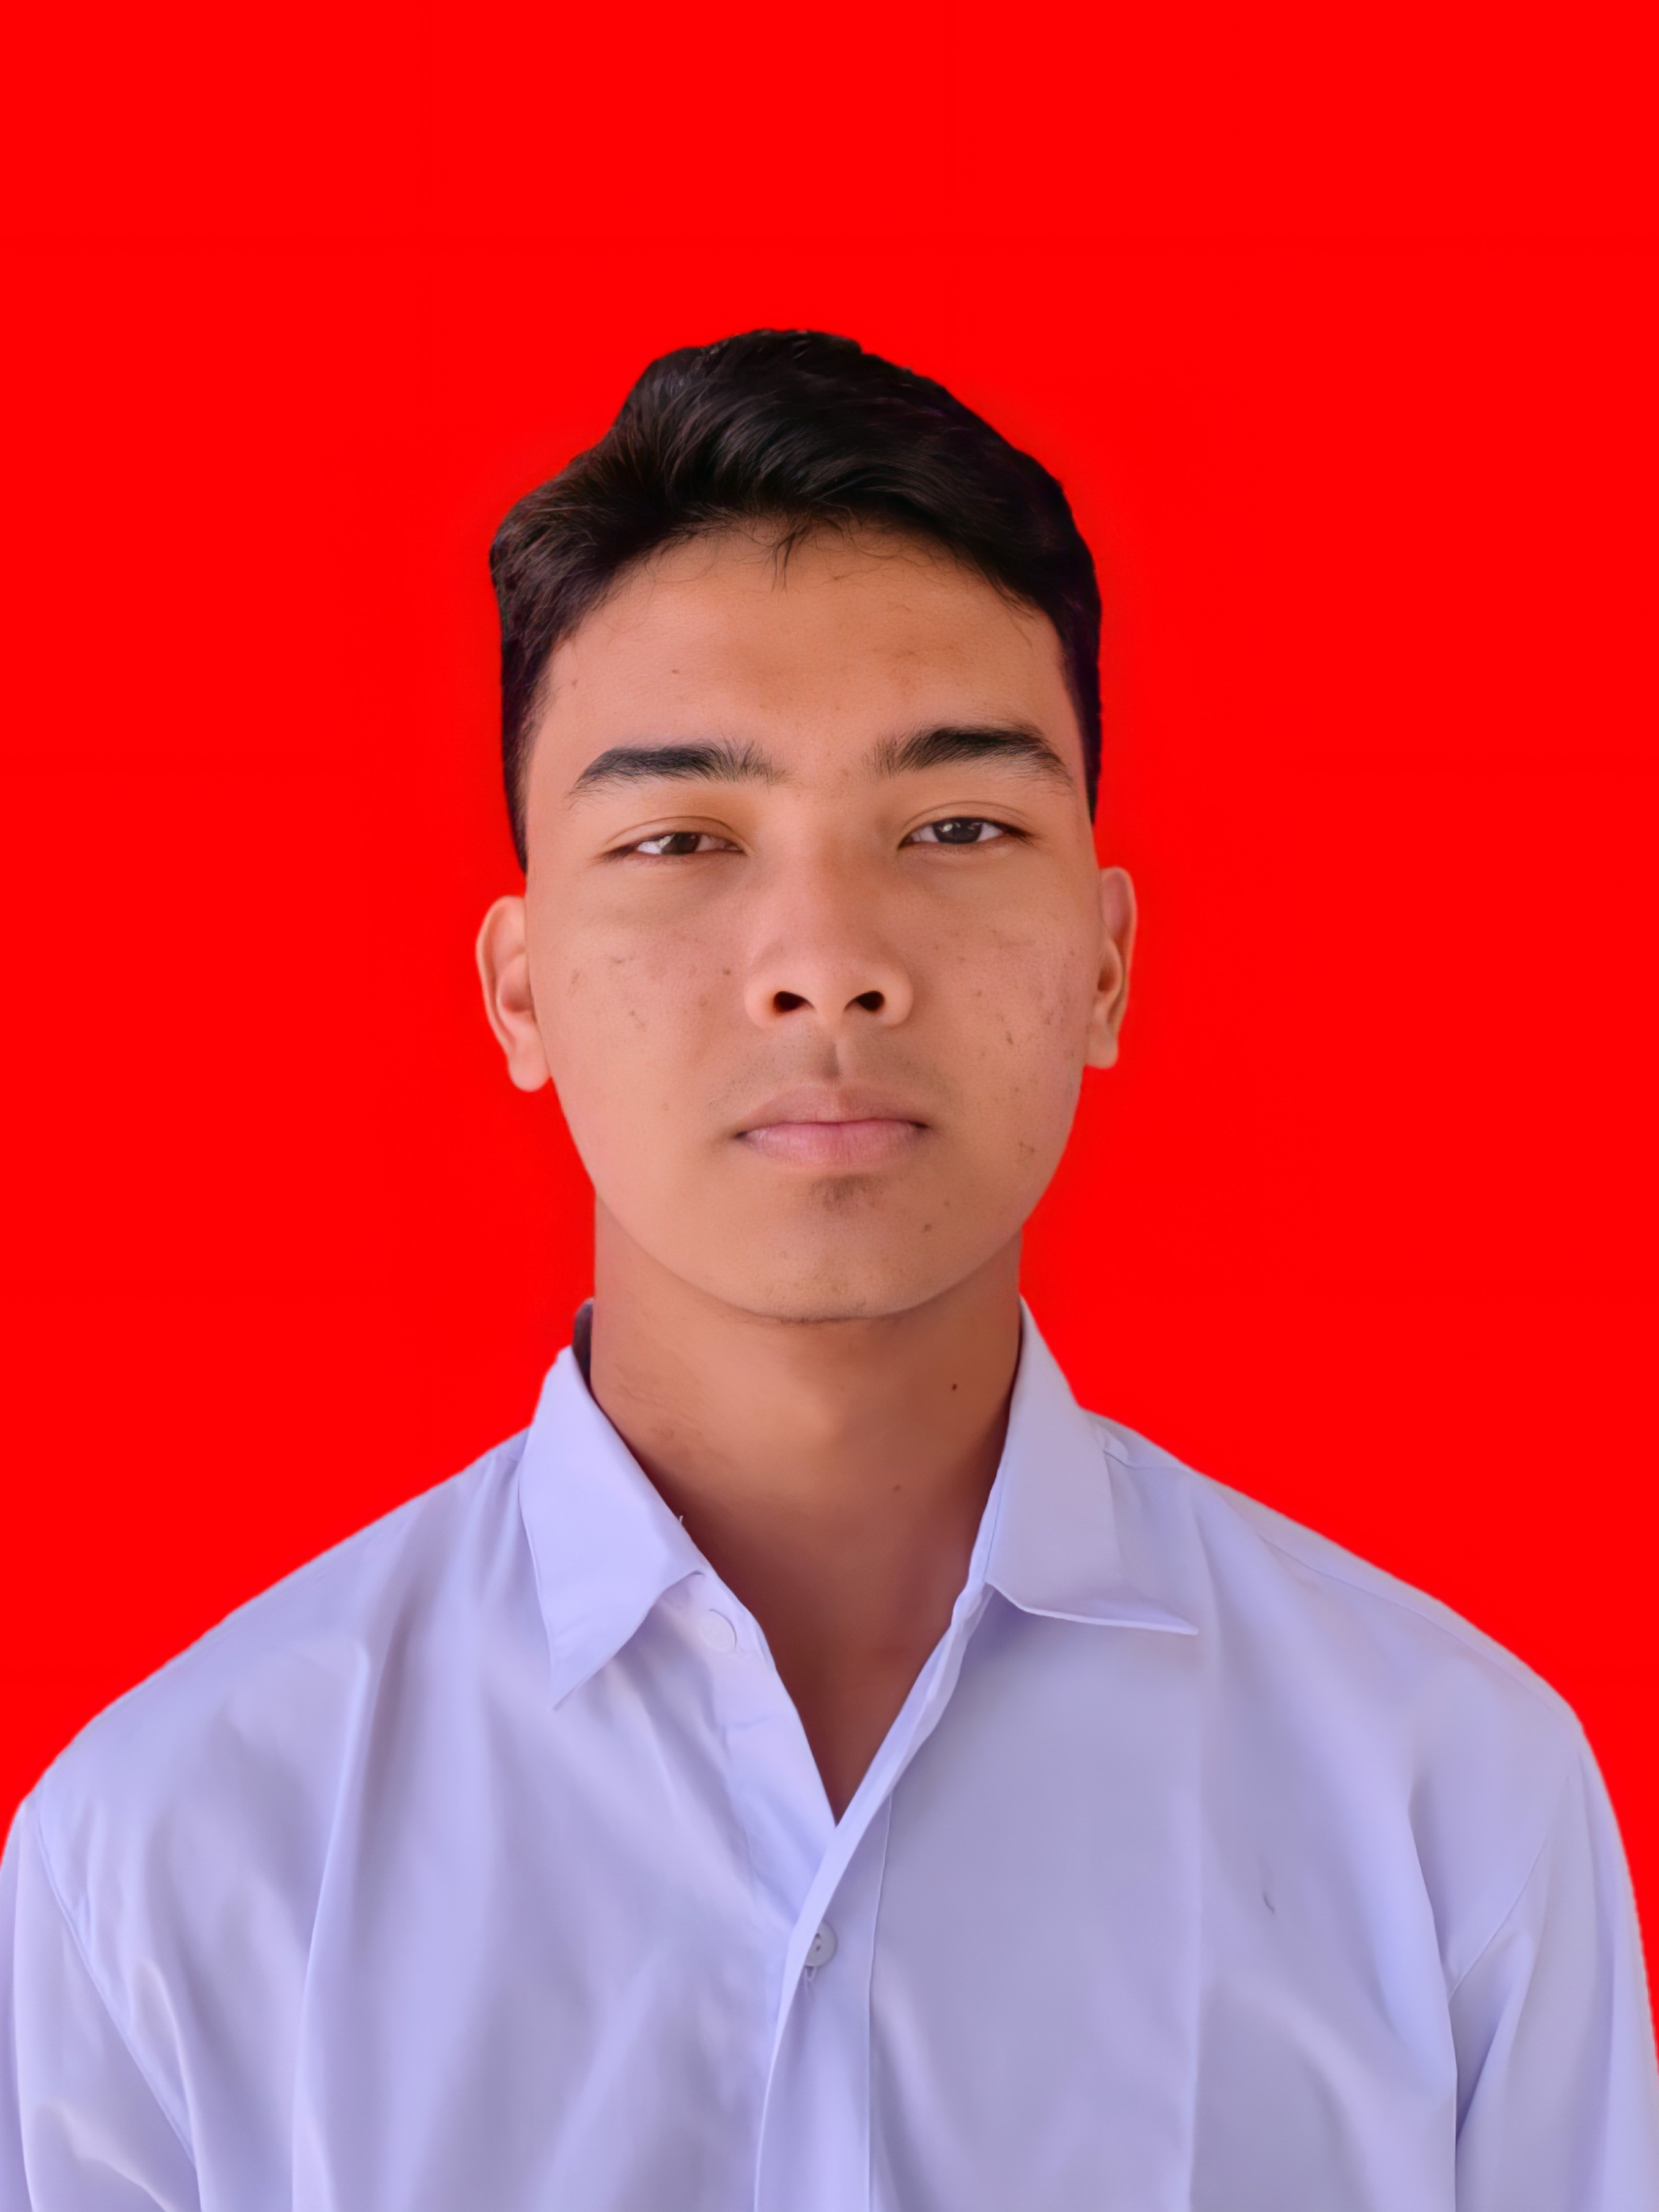
\includegraphics[width=3cm, height=4cm]{konten/gambar/fotoprofil.jpg}\vspace{-15pt}
\end{wrapfigure}
Hafiz Aryan Siregar lahir di Sibuhuan, pada tanggal 06 Desember 2002. Peneliti merupakan anak dari Bapak Almarhum Ahmad Sofyan Siregar dan Ibu Arni Shopiyah Nasution. Peneliti adalah anak pertama dari tiga bersaudara yang disebut anak panggoaran dalam istilah Mandailing. Pada tahun 2009 peneliti memulai pendidikan Sekolah Dasar di SD Negeri 0102 Sibuhuan. Setelah menyelesaikan pendidikan Sekolah Dasar peneliti melanjutkan pendidikan tingkat SLTP di MTs. Negeri Sibuhan dan selesai pada tahun 2018. Peneliti melanjutkan pendidikan di SMA Negeri 1 Barumun. Setelah menyelesaikan pendidikan di SMA Negeri 1 Barumun pada tahun 2021, peneliti pun melanjutkan pendidikan dengan menjadi mahasiswa Program Studi Sistem Informasi Fakultas Sains dan Teknologi Universitas Islam Negeri Sultan Syarif Kasim Riau. Pada masa perkuliahan, peneliti aktif berorganisasi dan menjadi bagian dari beberapa kepanitiaan. Peneliti bergabung di organisasi \textit{Information System Networking Club Research} (ISNC Research), Himpunan Mahasiswa Sistem Informasi (HIMASI) dan \textit{Google Developer Student Clubs} (GDSC). Peneliti aktif menjadi bagian dari Laboratorium Program Studi Sistem Informasi sebagai Asisten Laboratorium dan Tim Pengembang \textit{Website}. Tidak hanya belajar di dalam kelas, peneliti juga mengikuti program Merdeka Belajar Kampus Merdeka (MBKM) yaitu studi independen bersertifikat di Bangkit \textit{Academy} 2024 Batch 2 di alur belajar \textit{Cloud Computing}. Peneliti juga mengikuti \textit{Coding Camp powered by} DBS \textit{Foundation} 2025 di alur belajar \textit{Front-End} \& \textit{Back-End Developer} di akhir masa perkuliahan peneliti. Peneliti menyelesaikan pendidikan Strata-1 dalam waktu 8 semester setelah berhasil menyelesaikan Tugas Akhir (TA) dengan judul penelitian ”Pengembangan Sistem Informasi Manajemen Laboratorium Menggunakan Metode \textit{Agile Development}”.